\tikzset{every picture/.style={line width=0.75pt}} %set default line width to 0.75pt        

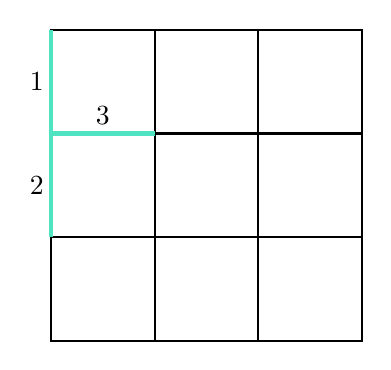
\begin{tikzpicture}[x=0.75pt,y=0.75pt,yscale=-1,xscale=1]
%uncomment if require: \path (0,300); %set diagram left start at 0, and has height of 300

%Shape: Square [id:dp9775774399102888] 
\draw   (169,58) -- (219,58) -- (219,108) -- (169,108) -- cycle ;
%Shape: Square [id:dp5803861188505348] 
\draw   (219,58) -- (269,58) -- (269,108) -- (219,108) -- cycle ;
%Shape: Square [id:dp7379150177319249] 
\draw   (169,108) -- (219,108) -- (219,158) -- (169,158) -- cycle ;
%Shape: Square [id:dp6254975238468878] 
\draw   (219,108) -- (269,108) -- (269,158) -- (219,158) -- cycle ;
%Shape: Square [id:dp9668425225055952] 
\draw   (269,58) -- (319,58) -- (319,108) -- (269,108) -- cycle ;
%Shape: Square [id:dp1445208133029452] 
\draw   (269,108) -- (319,108) -- (319,158) -- (269,158) -- cycle ;
%Shape: Square [id:dp06887087359110211] 
\draw   (169,158) -- (219,158) -- (219,208) -- (169,208) -- cycle ;
%Shape: Square [id:dp9361353940191639] 
\draw   (219,158) -- (269,158) -- (269,208) -- (219,208) -- cycle ;
%Shape: Square [id:dp8594572702460204] 
\draw   (269,158) -- (319,158) -- (319,208) -- (269,208) -- cycle ;
%Straight Lines [id:da3812400947940302] 
\draw [color={rgb, 255:red, 80; green, 227; blue, 194 }  ,draw opacity=1 ][line width=1.5]    (169,58) -- (169,108) ;
%Straight Lines [id:da5089201346271957] 
\draw [color={rgb, 255:red, 80; green, 227; blue, 194 }  ,draw opacity=1 ][line width=1.5]    (169,108) -- (169,158) ;
%Straight Lines [id:da12680120462207456] 
\draw [color={rgb, 255:red, 80; green, 227; blue, 194 }  ,draw opacity=1 ][line width=1.5]    (169,108) -- (219,108) ;

% Text Node
\draw (167,83) node [anchor=east] [inner sep=0.75pt]   [align=left] {1};
% Text Node
\draw (167,133) node [anchor=east] [inner sep=0.75pt]   [align=left] {2};
% Text Node
\draw (194,105) node [anchor=south] [inner sep=0.75pt]   [align=left] {3};


\end{tikzpicture}
